\documentclass[aspectratio=169,10pt]{beamer}

% ==============================================================================
% THEME & ADVANCED ACADEMIC VISUAL DESIGN
% ==============================================================================
\usetheme{Madrid}
\usecolortheme{whale}
\usefonttheme{professionalfonts}

% Premium Academic Palette
\definecolor{navyblue}{RGB}{0,32,96}
\definecolor{headerblue}{RGB}{12,38,92}
\definecolor{accentblue}{RGB}{20,68,140}
\definecolor{darkgreen}{RGB}{0,110,45}
\definecolor{crimsonred}{RGB}{160,18,18}
\definecolor{goldamber}{RGB}{210,120,0}
\definecolor{cardbg}{RGB}{248,250,253}
\definecolor{softblue}{RGB}{236,244,255}
\definecolor{softgreen}{RGB}{236,252,242}
\definecolor{softorange}{RGB}{255,246,232}
\definecolor{softred}{RGB}{255,240,240}
\definecolor{softpurple}{RGB}{246,240,255}
\definecolor{borderblue}{RGB}{35,85,160}
\definecolor{bordergreen}{RGB}{25,125,55}
\definecolor{borderorange}{RGB}{195,95,15}
\definecolor{borderred}{RGB}{165,35,35}
\definecolor{borderpurple}{RGB}{115,55,165}

% Beamer Element Colors
\setbeamercolor{palette primary}{bg=navyblue,fg=white}
\setbeamercolor{palette secondary}{bg=accentblue,fg=white}
\setbeamercolor{palette tertiary}{bg=headerblue,fg=white}
\setbeamercolor{frametitle}{bg=headerblue,fg=white}
\setbeamercolor{titlelike}{parent=palette primary}
\setbeamercolor{block title}{bg=accentblue,fg=white}
\setbeamercolor{block body}{bg=softblue,fg=black}
\setbeamercolor{block title example}{bg=darkgreen,fg=white}
\setbeamercolor{block body example}{bg=softgreen,fg=black}
\setbeamercolor{block title alerted}{bg=crimsonred,fg=white}
\setbeamercolor{block body alerted}{bg=softred,fg=black}

% Layout & Margins
\setbeamersize{text margin left=7mm, text margin right=7mm}
\setbeamertemplate{navigation symbols}{}
\setbeamertemplate{headline}{}

% Dynamic Footline
\setbeamertemplate{footline}{
    \leavevmode%
    \hbox{%
    \begin{beamercolorbox}[wd=.48\paperwidth,ht=2.5ex,dp=0.9ex,left]{palette primary}%
        \hspace*{3ex}\textbf{Verification Is All You Need (Dr.\ DINO)}
    \end{beamercolorbox}%
    \begin{beamercolorbox}[wd=.32\paperwidth,ht=2.5ex,dp=0.9ex,center]{palette secondary}%
        M.Sc. in Data Science -- HCMUS
    \end{beamercolorbox}%
    \begin{beamercolorbox}[wd=.20\paperwidth,ht=2.5ex,dp=0.9ex,right]{palette primary}%
        Slide \insertframenumber{} / \inserttotalframenumber\hspace*{3ex}
    \end{beamercolorbox}}%
    \vskip0pt%
}

% ==============================================================================
% PACKAGES
% ==============================================================================
\usepackage[utf8]{inputenc}
\usepackage[T1]{fontenc}
\usepackage[english]{babel}
\usepackage{amsmath,amssymb,amsfonts,mathtools,bm}
\usepackage{graphicx}
\usepackage{booktabs}
\usepackage{tikz}
\usetikzlibrary{shapes.geometric, arrows.meta, positioning, calc, fit, backgrounds, decorations.pathreplacing}

\graphicspath{{../output/}{output/}{../}{./}}

% Custom Stat Badge Macro
\newcommand{\statbadge}[3]{%
    \begin{tikzpicture}
        \node[draw=#2, fill=#2!10, rounded corners=4pt, inner sep=4.5pt, line width=0.8pt, align=center] {
            {\Large\textbf{\textcolor{#2}{#1}}}\\[2pt]
            {\scriptsize\textbf{#3}}
        };
    \end{tikzpicture}%
}

% ==============================================================================
% TITLE & METADATA
% ==============================================================================
\title[\textbf{Verification Is All You Need (Dr.\ DINO)}]{\textbf{\LARGE Verification Is All You Need:}\\[0.2em]\Large Emergent Object Discovery in Self-Supervised Vision Transformers via Dr.\ GRPO}
\subtitle{\normalsize Master of Science Thesis Defense in Data Science}
\author[Vu, Khang, Nam]{\textbf{Pham Cung Le Nhan Vu} \quad \textbf{Nguyen Hoang Khang} \quad \textbf{Nguyen Hoai Nam}}
\institute[HCMUS]{
    \textbf{Master of Science in Data Science} \\
    VNUHCM -- University of Science, Ho Chi Minh City, Vietnam
}
\date{\today}

\begin{document}

% ==============================================================================
% SLIDE 1: CUSTOM HERO TITLE SLIDE (WITH TEASER VISUALS & HOOK BADGES)
% ==============================================================================
\begin{frame}[plain]
\vspace{-0.6em}
% Title Banner
\begin{center}
    {\huge\textbf{\textcolor{navyblue}{Verification Is All You Need}}}\\[0.25em]
    {\large\textbf{Emergent Object Discovery in Self-Supervised Vision Transformers via Dr.\ GRPO}}\\[0.28em]
    {\footnotesize\textbf{Framework:} \textcolor{crimsonred}{\textbf{Dr.\ DINO}} \quad$\bm{\cdot}$\quad \textbf{Pham Cung Le Nhan Vu} \quad \textbf{Nguyen Hoang Khang} \quad \textbf{Nguyen Hoai Nam}}\\[0.18em]
    {\scriptsize\textit{Master of Science in Data Science} \quad$\bm{\cdot}$\quad \textbf{VNUHCM -- University of Science}}
\end{center}

\vspace{-0.35em}
\begin{columns}[c]
    % Left Column: Attention Teaser Banner (Showing Full Progression from Vanilla -> Stage 1 Base -> Stage 2 Full with Dr. GRPO)
    \begin{column}{0.64\textwidth}
        \begin{block}{\textbf{Visual Teaser: Emergent Object Discovery via Dr.\ GRPO}}
            \centering
            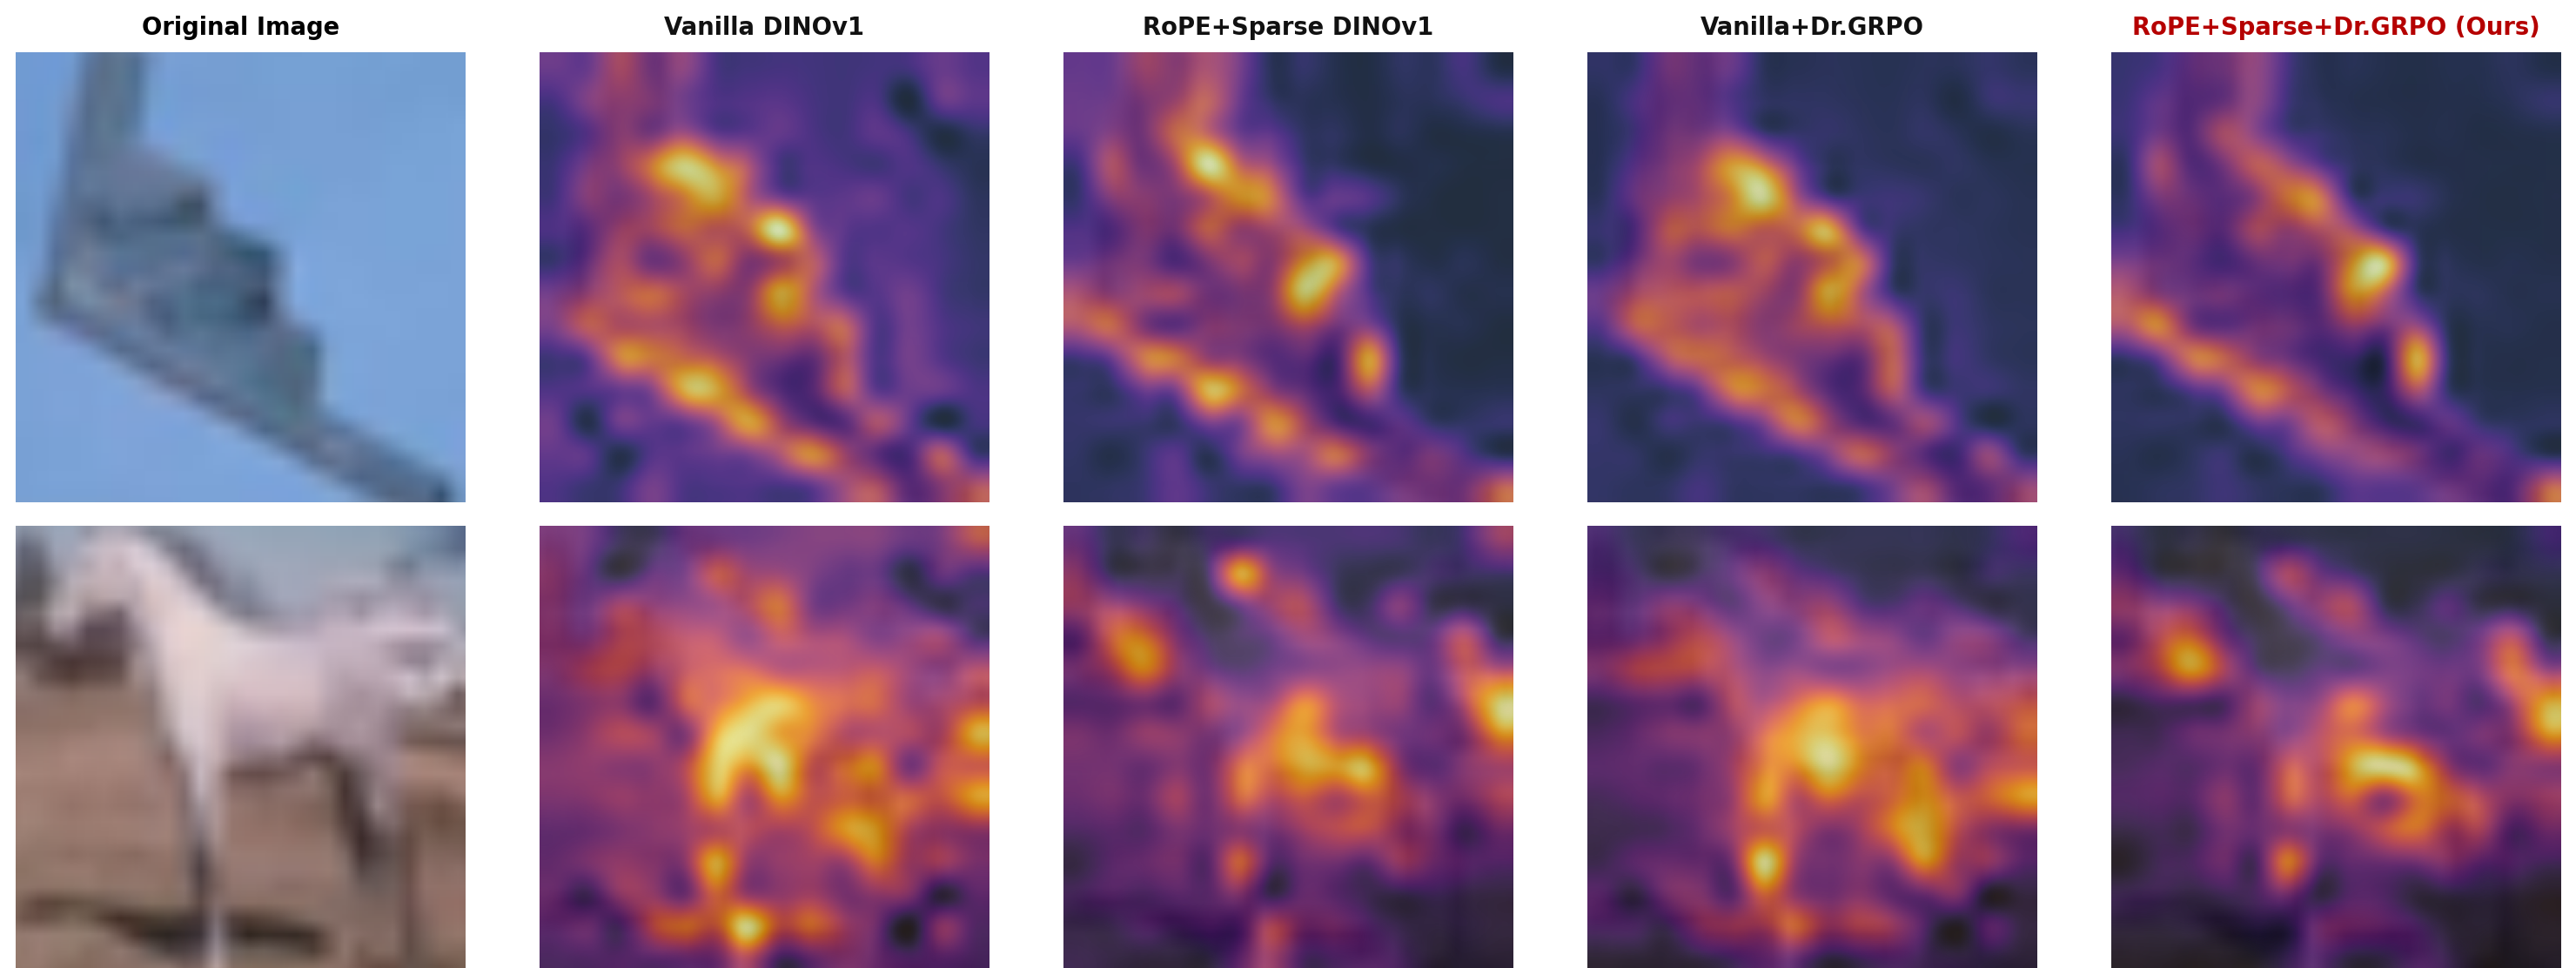
\includegraphics[width=\linewidth]{output/slide1_teaser_grid.png}
        \end{block}
        \vspace{-0.3em}
        \centering\scriptsize
        \textbf{Stage 1 (RoPE+Sparse Base):} Continuous geometry resolves sharp local sub-parts.\\
        \textcolor{darkgreen}{\textbf{Stage 2 (+ Dr.\ GRPO Alignment):}} RLVR purges background noise, boosting IoU by \textbf{+20.10\%}!
    \end{column}

    % Right Column: 4 Curiosity-Hook Stat Badges
    \begin{column}{0.34\textwidth}
        \centering
        \statbadge{+20.10\%}{darkgreen}{Foreground Mask IoU}\\[2.5pt]
        \statbadge{99.91\%}{accentblue}{Unsupervised CorLoc}\\[2.5pt]
        \statbadge{0 Overhead}{crimsonred}{Exact 21.67M Params}\\[2.5pt]
        \statbadge{< 3\,GB}{borderpurple}{RLVR VRAM Footprint}
    \end{column}
\end{columns}
\end{frame}

% ==============================================================================
% SLIDE 2: THE DEFENSE HOOK & EXECUTIVE HIGHLIGHTS
% ==============================================================================
\begin{frame}{Executive Highlights: Solving Vision Transformer Bottlenecks}
\vspace{-0.4em}
\begin{columns}[c]
    \begin{column}{0.58\textwidth}
        \textbf{\large The Fundamental Research Question:}
        \begin{itemize}\setlength{\itemsep}{2pt}
            \item \textit{Can Vision Transformers learn exact 2D geometry and discover object contours without human labels, without neural reward models, and with zero added parameters?}
        \end{itemize}

        \vspace{0.3em}
        \textbf{\large The Dr.\ DINO Architecture Paradigm:}
        \begin{enumerate}\setlength{\itemsep}{1pt}
            \item \textbf{Frequency-Adaptive 2D RoPE}: continuous relative geometry.
            \item \textbf{Spatial-Semantic Sparse Attention}: $-86.8\%$ computation.
            \item \textbf{Verifiable Dr.\ GRPO Alignment}: label-free RLVR.
        \end{enumerate}
    \end{column}

    \begin{column}{0.40\textwidth}
        \centering
        \statbadge{+20.10\%}{darkgreen}{Foreground Mask IoU}\\[2pt]
        \statbadge{99.91\%}{accentblue}{Unsupervised CorLoc}\\[2pt]
        \statbadge{0 Overhead}{crimsonred}{Exact 21.67M Params}\\[2pt]
        \statbadge{< 3\,GB}{borderpurple}{RLVR VRAM Footprint}
    \end{column}
\end{columns}

\vspace{0.2em}
\begin{exampleblock}{\textbf{Core Breakthrough}}
    \centering\small
    \textbf{83.98\%} Linear Probe Top-1 (+2.52\%) and \textbf{75.97\%} $k$-NN Top-1 (+1.56\%) on CIFAR-10 with \textbf{exact parameter parity}!
\end{exampleblock}
\end{frame}

% ==============================================================================
% SLIDE 3: DINOv1 FOUNDATION: SELF-DISTILLATION ARCHITECTURE
% ==============================================================================
\begin{frame}{The Foundation: DINOv1 Self-Distillation Framework}
\vspace{-0.4em}
\textbf{DINO} (\textbf{DI}stillation with \textbf{NO} labels -- Caron et al., Meta AI, ICCV 2021) revolutionized self-supervised learning:

\vspace{0.2em}
\begin{columns}[c]
    % Column 1: TikZ Framework Pipeline
    \begin{column}{0.54\textwidth}
        \centering
        \resizebox{\linewidth}{!}{%
        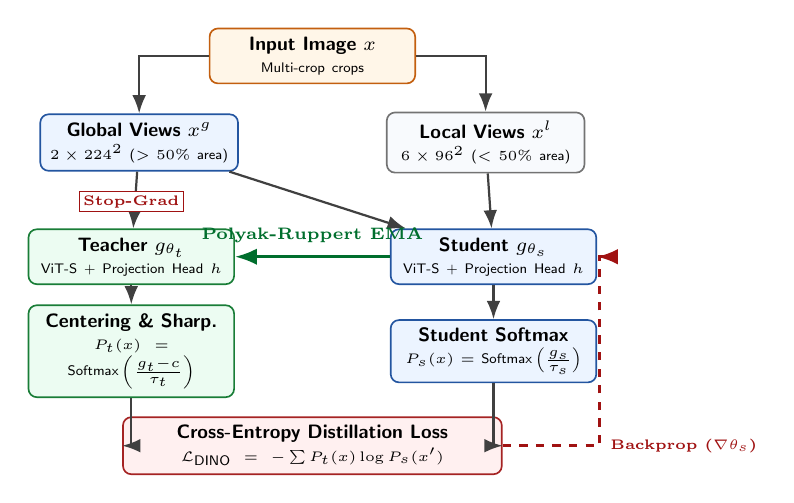
\begin{tikzpicture}[
            font=\sffamily\scriptsize,
            >=Latex,
            box/.style={draw=black!70, rounded corners=3pt, align=center, inner sep=3pt, line width=0.6pt},
            bluebox/.style={box, fill=softblue, draw=borderblue},
            greenbox/.style={box, fill=softgreen, draw=bordergreen},
            redbox/.style={box, fill=softred, draw=borderred},
            graybox/.style={box, fill=cardbg, draw=black!55},
            arrow/.style={->, line width=0.8pt, draw=black!75}
        ]
            % Image Input
            \node[box, fill=softorange, draw=borderorange, text width=2.4cm] (img) at (0, 2.5) {\textbf{Input Image $x$}\\ \tiny Multi-crop crops};
            
            % Global & Local Views
            \node[bluebox, text width=2.3cm] (global) at (-2.2, 1.4) {\textbf{Global Views $x^g$}\\ \tiny $2\times 224^2$ ($>50\%$ area)};
            \node[graybox, text width=2.3cm] (local) at (2.2, 1.4) {\textbf{Local Views $x^l$}\\ \tiny $6\times 96^2$ ($<50\%$ area)};
            
            % Teacher and Student
            \node[greenbox, text width=2.4cm] (teacher) at (-2.3, -0.05) {\textbf{Teacher $g_{\theta_t}$}\\ \tiny ViT-S + Projection Head $h$};
            \node[bluebox, text width=2.4cm] (student) at (2.3, -0.05) {\textbf{Student $g_{\theta_s}$}\\ \tiny ViT-S + Projection Head $h$};
            
            % Arrows from Views
            \draw[arrow] (img) -| (global);
            \draw[arrow] (img) -| (local);
            \draw[arrow] (global) -- (teacher);
            \draw[arrow] (global) -- (student);
            \draw[arrow] (local) -- (student);
            
            % Centering / Sharpening & Softmax
            \node[greenbox, text width=2.4cm] (t_out) at (-2.3, -1.25) {\textbf{Centering \& Sharp.}\\ \tiny $P_t(x) = \text{Softmax}\left(\frac{g_t - c}{\tau_t}\right)$};
            \node[bluebox, text width=2.4cm] (s_out) at (2.3, -1.25) {\textbf{Student Softmax}\\ \tiny $P_s(x) = \text{Softmax}\left(\frac{g_s}{\tau_s}\right)$};
            
            \draw[arrow] (teacher) -- (t_out);
            \draw[arrow] (student) -- (s_out);
            
            % Loss
            \node[redbox, text width=4.6cm] (loss) at (0, -2.45) {\textbf{Cross-Entropy Distillation Loss}\\ \tiny $\mathcal{L}_{\text{DINO}} = -\sum P_t(x) \log P_s(x')$};
            \draw[arrow] (t_out) |- (loss);
            \draw[arrow] (s_out) |- (loss);
            
            % Updates
            \draw[arrow, crimsonred, dashed, line width=1pt] (loss) -| node[right, font=\tiny\bfseries] {Backprop ($\nabla \theta_s$)} (3.65, -0.05) -- (student);
            \draw[arrow, darkgreen, line width=1.1pt] (student) -- node[above=1pt, font=\fontsize{6.5pt}{7.5pt}\selectfont\bfseries] {Polyak-Ruppert EMA} (teacher);
            \node[draw=crimsonred, fill=white, inner sep=1.5pt, font=\tiny\bfseries, text=crimsonred] at (-2.3, 0.65) {Stop-Grad};
        \end{tikzpicture}%
        }
    \end{column}

    % Column 2: Core Architecture Pillars
    \begin{column}{0.45\textwidth}
        \begin{block}{\textbf{Student--Teacher Dynamics}}
            \small
            \begin{itemize}\setlength{\itemsep}{2pt}
                \item \textbf{Identical Architecture}: Both networks share a ViT backbone and 3-layer MLP ($K=65,536$ dims).
                \item \textbf{Online Momentum Teacher}: Updated strictly via Polyak-Ruppert EMA ($\lambda \in [0.996, 1.0]$) with \textbf{no backpropagation}.
            \end{itemize}
        \end{block}
        
        \vspace{0.2em}
        \begin{exampleblock}{\textbf{Local-to-Global Induction}}
            \small
            Teacher sees only \textbf{global scenes}; Student must predict the whole scene from \textbf{small local glimpses}.
        \end{exampleblock}
    \end{column}
\end{columns}
\end{frame}

% ==============================================================================
% SLIDE 4: DINOv1 MATHEMATICS: COLLAPSE PREVENTION
% ==============================================================================
\begin{frame}{DINOv1 Mechanics: Centering, Sharpening \& Loss}
\vspace{-0.5em}
Unlike contrastive methods (SimCLR, MoCo), DINO requires \textbf{no negative pairs}. How does it avoid collapse?

\vspace{0.1em}
\begin{columns}[t]
    % Column 1: Centering vs Sharpening
    \begin{column}{0.49\textwidth}
        \begin{alertblock}{\textbf{Centering (Prevents Dominance)}}
            \footnotesize
            Subtracts dynamic EMA center vector $\mathbf{c} \in \mathbb{R}^K$:
            \begin{align*}
                g_t(x) &\leftarrow g_t(x) - \mathbf{c} \\
                \mathbf{c} &\leftarrow m \mathbf{c} + (1 - m) \tfrac{1}{B} \sum_{i=1}^B g_{\theta_t}(x_i)
            \end{align*}
            \vspace{-0.7em}
            \begin{itemize}\setlength{\itemsep}{0pt}
                \item Pulls predictions towards uniform.
                \item Prevents collapse to a single dimension!
            \end{itemize}
        \end{alertblock}
    \end{column}

    % Column 2: Sharpening
    \begin{column}{0.49\textwidth}
        \begin{exampleblock}{\textbf{Sharpening (Prevents Uniformity)}}
            \footnotesize
            Uses asymmetric temperatures ($\tau_t \ll \tau_s$):
            \[
                P_t(x)^{(k)} = \frac{\exp\big((g_{\theta_t}(x)^{(k)} - c^{(k)}) / \tau_t\big)}{\sum_{j=1}^K \exp\big((g_{\theta_t}(x)^{(j)} - c^{(j)}) / \tau_t\big)}
            \]
            \vspace{-0.7em}
            \begin{itemize}\setlength{\itemsep}{0pt}
                \item $\tau_s = 0.1$, while $\tau_t \in [0.04, 0.07]$.
                \item Low temperature sharpens peak probability.
                \item Prevents collapse to uniform entropy!
            \end{itemize}
        \end{exampleblock}
    \end{column}
\end{columns}

\vspace{0.2em}
\begin{block}{\textbf{Dynamic Thermodynamic Equilibrium}}
    \centering\footnotesize
    $\mathbf{c}$ acts as a repulsive center force; low $\tau_t$ acts as an attractive sharpening force.\\
    Their interaction guarantees stable, non-collapsed representation learning without contrastive negatives.
\end{block}
\end{frame}

% ==============================================================================
% SLIDE 5: DINOv1 BREAKTHROUGH: EMERGENT PROPERTIES IN ViTs
% ==============================================================================
\begin{frame}{The Breakthrough of DINOv1: Emergent Properties in ViTs}
\vspace{-0.4em}
Prior to DINO, self-supervised learning flourished on CNNs but failed to scale cleanly on Vision Transformers:

\vspace{0.2em}
\begin{columns}[t]
    % Column 1: Unsupervised Object Segmentation
    \begin{column}{0.49\textwidth}
        \begin{exampleblock}{\textbf{1. Emergent Object Segmentation}}
            \small
            \begin{itemize}\setlength{\itemsep}{2pt}
                \item \textbf{Explicit Scene De-occlusion}: Self-attention maps of the last-layer \texttt{[CLS]} token segment physical object boundaries \textbf{completely without supervision}.
                \item \textbf{Head Specialization}: Different heads naturally capture foreground objects, textures, and background contours without any human bounding boxes.
            \end{itemize}
        \end{exampleblock}
    \end{column}

    % Column 2: Linear & k-NN Separability
    \begin{column}{0.49\textwidth}
        \begin{block}{\textbf{2. High-Quality Semantic Clustering}}
            \small
            \begin{itemize}\setlength{\itemsep}{2pt}
                \item \textbf{High-Performance $k$-NN}: Direct $k$-nearest neighbor classification on frozen ViT features achieves \textbf{78.3\%} Top-1 on ImageNet-1K without fine-tuning.
                \item \textbf{Geometric Semantics}: Feature manifolds group semantically related concepts together.
            \end{itemize}
        \end{block}
    \end{column}
\end{columns}

\vspace{0.3em}
\begin{alertblock}{\textbf{The Unsolved Dilemma: Why DINOv1 Needs Enhancement}}
    \centering\small
    Despite this brilliance, standard DINOv1 ViTs suffer from \textbf{coordinate warping under multi-crop}, \textbf{quadratic attention dilution}, and \textbf{residual background halos}.
\end{alertblock}
\end{frame}

% ==============================================================================
% SLIDE 6: VISUAL BREAKDOWN OF THE 3 BOTTLENECKS
% ==============================================================================
\begin{frame}{The Problem: 3 Structural Flaws in Vanilla DINOv1}
\vspace{-0.3em}
\begin{columns}[t]
    % Flaw 1
    \begin{column}{0.32\textwidth}
        \begin{alertblock}{\textbf{1. Multi-Crop Warping}}
            \centering
            \vspace{0.2em}
            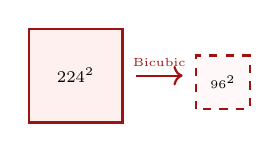
\begin{tikzpicture}[scale=0.85, every node/.style={transform shape}]
                \draw[thick, draw=crimsonred, fill=softred] (0,0) rectangle (1.4,1.4) node[pos=0.5, font=\scriptsize\bfseries] {$224^2$};
                \draw[->, thick, crimsonred] (1.6,0.7) -- node[above, font=\tiny] {Bicubic} (2.3,0.7);
                \draw[thick, dashed, draw=crimsonred, fill=softred!50] (2.5,0.2) rectangle (3.3,1.0) node[pos=0.5, font=\tiny\bfseries] {$96^2$};
            \end{tikzpicture}
            \vspace{0.2em}
            \footnotesize
            \begin{itemize}\setlength{\itemsep}{1pt}
                \item Static APEs warped by interpolation.
                \item Destroys relative spatial phase.
            \end{itemize}
        \end{alertblock}
    \end{column}

    % Flaw 2
    \begin{column}{0.32\textwidth}
        \begin{alertblock}{\textbf{2. Attention Dilution}}
            \centering
            \vspace{0.2em}
            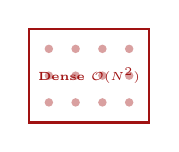
\begin{tikzpicture}[scale=0.85, every node/.style={transform shape}]
                \draw[thick, draw=crimsonred, fill=white] (0,0) rectangle (1.8,1.4);
                \foreach \x in {0.3, 0.7, 1.1, 1.5} {
                    \foreach \y in {0.3, 0.7, 1.1} {
                        \fill[crimsonred!40] (\x,\y) circle (1.8pt);
                    }
                }
                \node[font=\tiny\bfseries, text=crimsonred] at (0.9, 0.7) {Dense $\mathcal{O}(N^2)$};
            \end{tikzpicture}
            \vspace{0.2em}
            \footnotesize
            \begin{itemize}\setlength{\itemsep}{1pt}
                \item $>85\%$ weights near zero.
                \item Background (sky/grass) pollutes \texttt{[CLS]}.
            \end{itemize}
        \end{alertblock}
    \end{column}

    % Flaw 3
    \begin{column}{0.32\textwidth}
        \begin{alertblock}{\textbf{3. Background Leakage}}
            \centering
            \vspace{0.2em}
            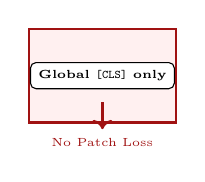
\begin{tikzpicture}[scale=0.85, every node/.style={transform shape}]
                \draw[thick, draw=crimsonred, fill=softred] (0,0) rectangle (2.2,1.4);
                \node[draw=black, fill=white, rounded corners=2pt, font=\tiny\bfseries] at (1.1, 0.7) {Global \texttt{[CLS]} only};
                \draw[->, thick, crimsonred] (1.1, 0.3) -- (1.1, -0.1) node[below, font=\tiny] {No Patch Loss};
            \end{tikzpicture}
            \vspace{0.2em}
            \footnotesize
            \begin{itemize}\setlength{\itemsep}{1pt}
                \item Global CE ignores spatial masks.
                \item Residual noise persists indefinitely.
            \end{itemize}
        \end{alertblock}
    \end{column}
\end{columns}

\vspace{0.4em}
\begin{block}{\textbf{Dr.\ DINO Paradigm Shift}}
    \centering\small
    \textbf{Continuous Geometry (2D RoPE)} \quad $\bm{\oplus}$ \quad \textbf{Focused Routing (S$^3$ Attention)} \quad $\bm{\oplus}$ \quad \textbf{Verifiable RLVR (Dr.\ GRPO)}
\end{block}
\end{frame}

% ==============================================================================
% SLIDE 4: ARCHITECTURAL COMPARISON (TIKZ)
% ==============================================================================
\begin{frame}{Architectural Blueprint: Baseline vs. Dr.\ DINO Block}
\vspace{-0.3em}
\begin{columns}[c]
    \begin{column}{0.62\textwidth}
        \centering
        \resizebox{\textwidth}{!}{%
        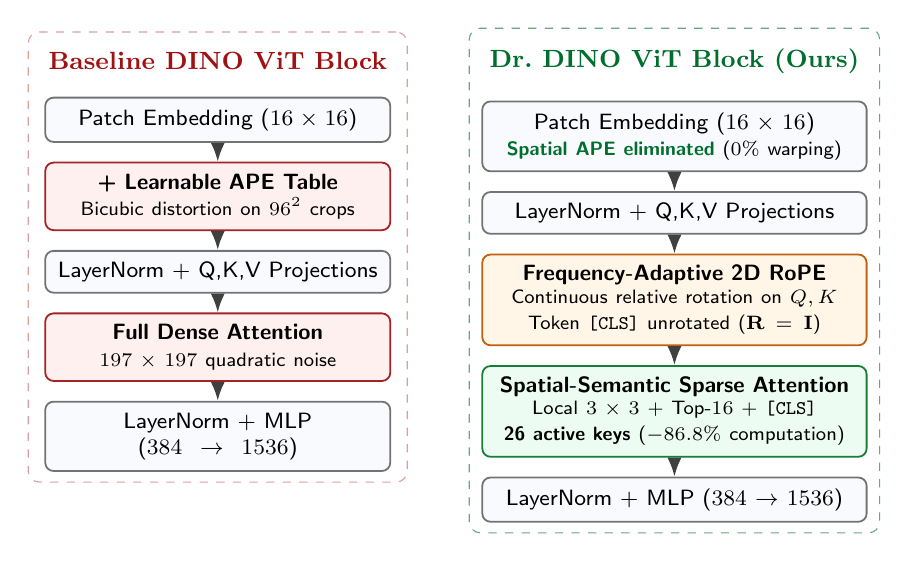
\begin{tikzpicture}[
            font=\sffamily\footnotesize,
            >=Latex,
            box/.style={draw=black!70, rounded corners=3pt, align=center, inner sep=4pt, line width=0.65pt},
            bluebox/.style={box, fill=softblue, draw=borderblue},
            greenbox/.style={box, fill=softgreen, draw=bordergreen},
            orangebox/.style={box, fill=softorange, draw=borderorange},
            redbox/.style={box, fill=softred, draw=borderred},
            graybox/.style={box, fill=cardbg, draw=black!55},
            arrow/.style={->, line width=0.85pt, draw=black!75}
        ]
            % Baseline Block
            \begin{scope}[local bounding box=colBase]
                \node[font=\bfseries\small, text=crimsonred] (tb) at (0, 0) {Baseline DINO ViT Block};
                \node[graybox, text width=4.1cm, below=0.22cm of tb] (b1) {Patch Embedding ($16\times 16$)};
                \node[redbox, text width=4.1cm, below=0.24cm of b1] (b2) {\textbf{+ Learnable APE Table}\\ \scriptsize Bicubic distortion on $96^2$ crops};
                \node[graybox, text width=4.1cm, below=0.24cm of b2] (b3) {LayerNorm + Q,K,V Projections};
                \node[redbox, text width=4.1cm, below=0.24cm of b3] (b4) {\textbf{Full Dense Attention}\\ \scriptsize $197\times 197$ quadratic noise};
                \node[graybox, text width=4.1cm, below=0.24cm of b4] (b5) {LayerNorm + MLP ($384\to 1536$)};
                \draw[arrow] (b1) -- (b2);
                \draw[arrow] (b2) -- (b3);
                \draw[arrow] (b3) -- (b4);
                \draw[arrow] (b4) -- (b5);
            \end{scope}

            % Dr. DINO Block
            \begin{scope}[local bounding box=colProp, xshift=5.8cm]
                \node[font=\bfseries\small, text=darkgreen] (tp) at (0, 0) {Dr.\ DINO ViT Block (Ours)};
                \node[graybox, text width=4.6cm, below=0.22cm of tp] (p1) {Patch Embedding ($16\times 16$)\\ \scriptsize \textcolor{darkgreen}{\textbf{Spatial APE eliminated}} ($0\%$ warping)};
                \node[graybox, text width=4.6cm, below=0.24cm of p1] (p2) {LayerNorm + Q,K,V Projections};
                \node[orangebox, text width=4.6cm, below=0.24cm of p2] (p3) {\textbf{Frequency-Adaptive 2D RoPE}\\ \scriptsize Continuous relative rotation on $Q, K$\\ \scriptsize Token \texttt{[CLS]} unrotated ($\mathbf{R}=\mathbf{I}$)};
                \node[greenbox, text width=4.6cm, below=0.24cm of p3] (p4) {\textbf{Spatial-Semantic Sparse Attention}\\ \scriptsize Local $3\times 3$ + Top-$16$ + \texttt{[CLS]}\\ \scriptsize \textbf{26 active keys} ($-86.8\%$ computation)};
                \node[graybox, text width=4.6cm, below=0.24cm of p4] (p5) {LayerNorm + MLP ($384\to 1536$)};
                \draw[arrow] (p1) -- (p2);
                \draw[arrow] (p2) -- (p3);
                \draw[arrow] (p3) -- (p4);
                \draw[arrow] (p4) -- (p5);
            \end{scope}

            \begin{scope}[on background layer]
                \node[draw=crimsonred!40, dashed, rounded corners=4pt, fit=(colBase), inner sep=4pt] {};
                \node[draw=darkgreen!60, dashed, rounded corners=4pt, fit=(colProp), inner sep=4pt] {};
            \end{scope}
        \end{tikzpicture}%
        }
    \end{column}

    \begin{column}{0.37\textwidth}
        \begin{block}{\textbf{Strict Zero-Overhead Guarantee}}
            \small
            \begin{itemize}\setlength{\itemsep}{3pt}
                \item \textbf{Parameters}: Exactly \textbf{21,665,664} (0\% parameter inflation).
                \item \textbf{FLOPs}: Exactly \textbf{9.20 GFLOPs} (identical theoretical complexity).
                \item \textbf{Translation Invariance}: Continuous spatial displacement $(\Delta x, \Delta y)$ directly encoded!
            \end{itemize}
        \end{block}
        
        \vspace{0.2em}
        \begin{exampleblock}{\textbf{Scientific Rigor}}
            \small
            Performance gains arise purely from geometric inductive bias, not model capacity inflation!
        \end{exampleblock}
    \end{column}
\end{columns}
\end{frame}

% ==============================================================================
% SLIDE 5: INNOVATION 1 — FREQUENCY-ADAPTIVE 2D RoPE (MATH MADE VISUAL)
% ==============================================================================
\begin{frame}{Innovation 1: Frequency-Adaptive 2D RoPE (Math Made Visual)}
\vspace{-0.5em}
\begin{columns}[c]
    % Visual TikZ Diagram of 2D RoPE
    \begin{column}{0.48\textwidth}
        \centering
        \resizebox{0.85\textwidth}{!}{%
        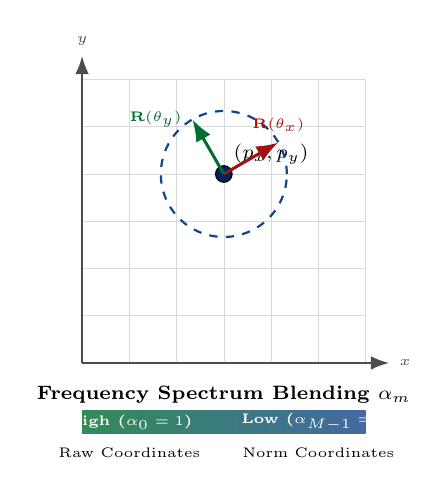
\begin{tikzpicture}[font=\sffamily\footnotesize, >=Latex]
            % 2D Grid Coordinate
            \draw[step=0.6cm, gray!30, very thin] (0,0) grid (3.6,3.6);
            \draw[->, thick, black!70] (0,0) -- (3.9,0) node[right, font=\tiny] {$x$};
            \draw[->, thick, black!70] (0,0) -- (0,3.9) node[above, font=\tiny] {$y$};

            % Patch coordinate
            \filldraw[fill=navyblue, draw=black] (1.8, 2.4) circle (3pt) node[above right, font=\scriptsize\bfseries] {$(p_x, p_y)$};

            % Rotation circle
            \draw[dashed, draw=accentblue, line width=0.8pt] (1.8, 2.4) circle (0.8cm);
            \draw[->, line width=1.1pt, crimsonred] (1.8, 2.4) -- ++(30:0.8cm) node[above, font=\tiny\bfseries] {$\mathbf{R}(\theta_x)$};
            \draw[->, line width=1.1pt, darkgreen] (1.8, 2.4) -- ++(120:0.8cm) node[left, font=\tiny\bfseries] {$\mathbf{R}(\theta_y)$};

            % Frequency Spectrum Ramp
            \node[font=\scriptsize\bfseries] at (1.8, -0.4) {Frequency Spectrum Blending $\alpha_m$};
            \shade[left color=darkgreen!80, right color=accentblue!80] (0, -0.9) rectangle (3.6, -0.6);
            \node[font=\tiny\bfseries, text=white] at (0.6, -0.75) {High ($\alpha_0=1$)};
            \node[font=\tiny\bfseries, text=white] at (3.0, -0.75) {Low ($\alpha_{M-1}=0$)};
            \node[font=\tiny, below=0.1cm of {0.6, -0.85}] {Raw Coordinates};
            \node[font=\tiny, below=0.1cm of {3.0, -0.85}] {Norm Coordinates};
        \end{tikzpicture}%
        }
    \end{column}

    % Math & Properties
    \begin{column}{0.50\textwidth}
        \begin{block}{\textbf{Rotary Equivariance Inner Product}}
            \small
            \vspace{-0.2em}
            \[ \langle \tilde{\mathbf{q}}_i, \tilde{\mathbf{k}}_j \rangle = \mathbf{q}_i^\top \mathbf{R}_{\Theta}(p_{x,i}-p_{x,j}, \, p_{y,i}-p_{y,j}) \mathbf{k}_j \]
            \vspace{-0.3em}
            \scriptsize Relative displacement $(\Delta x, \Delta y)$ is preserved exactly!
        \end{block}

        \vspace{-0.2em}
        \begin{exampleblock}{\textbf{Continuous Coordinate Blending}}
            \small
            \vspace{-0.2em}
            \[ p_m = \alpha_m \cdot p_{\text{raw}} + (1 - \alpha_m) \cdot p_{\text{norm}}, \quad \alpha_m = 1 - \frac{m}{M-1} \]
            \vspace{-0.4em}
            \begin{itemize}\setlength{\itemsep}{2pt}
                \item \textbf{High Frequencies}: Preserve sharp local boundaries.
                \item \textbf{Low Frequencies}: Scale invariance across multi-crop views.
                \item \textbf{\texttt{[CLS]} Token}: $\boldsymbol{\theta}_{\text{cls}} = \mathbf{0} \implies \mathbf{R}=\mathbf{I}$ (unbiased global view).
            \end{itemize}
        \end{exampleblock}
    \end{column}
\end{columns}
\end{frame}

% ==============================================================================
% SLIDE 6: INNOVATION 2 — SPATIAL-SEMANTIC SPARSE ATTENTION
% ==============================================================================
\begin{frame}{Innovation 2: Spatial-Semantic Sparse Softmax Attention}
\vspace{-0.2em}
\begin{columns}[c]
    \begin{column}{0.48\textwidth}
        \centering
        \resizebox{0.88\textwidth}{!}{%
        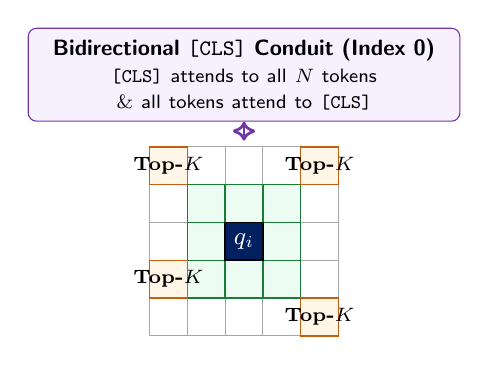
\begin{tikzpicture}[
            font=\sffamily\footnotesize,
            box/.style={draw=black!70, rounded corners=3pt, align=center, inner sep=4pt}
        ]
            \node[box, fill=softpurple, draw=borderpurple, text width=5.2cm] (cls) {
                \textbf{Bidirectional \texttt{[CLS]} Conduit (Index 0)}\\
                \scriptsize \texttt{[CLS]} attends to all $N$ tokens $\&$ all tokens attend to \texttt{[CLS]}
            };

            \coordinate (gtop) at ([yshift=-0.32cm]cls.south);
            \def\cs{0.48}
            \begin{scope}[shift={($(gtop)+(-2.5*\cs, -5*\cs)$)}]
                \foreach \r in {0,...,4} {
                    \foreach \c in {0,...,4} {
                        \filldraw[fill=white, draw=black!35, line width=0.4pt]
                            (\c*\cs, \r*\cs) rectangle ++(\cs, \cs);
                    }
                }
                \foreach \r in {1,2,3} {
                    \foreach \c in {1,2,3} {
                        \filldraw[fill=softgreen, draw=bordergreen, line width=0.55pt]
                            (\c*\cs, \r*\cs) rectangle ++(\cs, \cs);
                    }
                }
                \filldraw[fill=navyblue, draw=black, line width=0.7pt]
                    (2*\cs, 2*\cs) rectangle ++(\cs, \cs)
                    node[pos=0.5, text=white, font=\bfseries\small] {$q_i$};
                \filldraw[fill=softorange, draw=borderorange, line width=0.55pt]
                    (0*\cs, 4*\cs) rectangle ++(\cs, \cs) node[pos=0.5, font=\scriptsize\bfseries] {Top-$K$};
                \filldraw[fill=softorange, draw=borderorange, line width=0.55pt]
                    (4*\cs, 4*\cs) rectangle ++(\cs, \cs) node[pos=0.5, font=\scriptsize\bfseries] {Top-$K$};
                \filldraw[fill=softorange, draw=borderorange, line width=0.55pt]
                    (4*\cs, 0*\cs) rectangle ++(\cs, \cs) node[pos=0.5, font=\scriptsize\bfseries] {Top-$K$};
                \filldraw[fill=softorange, draw=borderorange, line width=0.55pt]
                    (0*\cs, 1*\cs) rectangle ++(\cs, \cs) node[pos=0.5, font=\scriptsize\bfseries] {Top-$K$};
            \end{scope}

            \draw[<->, line width=1.0pt, draw=borderpurple] (cls.south) -- ++(0, -0.24);
        \end{tikzpicture}%
        }
    \end{column}

    \begin{column}{0.50\textwidth}
        \begin{block}{\textbf{Active Support $\mathcal{S}_i$: Exactly 26 Keys}}
            \small
            \begin{itemize}\setlength{\itemsep}{2pt}
                \item \textcolor{bordergreen}{\textbf{Local Window $\mathcal{N}_{\text{local}}$}}: $3\times 3$ spatial neighborhood ($9$ keys).
                \item \textcolor{borderorange}{\textbf{Semantic Top-$16$ $\mathcal{N}_{\text{semantic}}$}}: dynamic content routing across distant tokens ($16$ keys).
                \item \textcolor{borderpurple}{\textbf{Bidirectional \texttt{[CLS]}}}: global context conduit ($1$ key).
            \end{itemize}
            \centering \textbf{86.8\% Computation Reduction} ($26 / 197$ keys).
        \end{block}
        
        \vspace{-0.2em}
        \begin{exampleblock}{\textbf{Exact Softmax Normalization}}
            \small
            \vspace{-0.3em}
            \[ \mathbf{A}_{ij} = \frac{\exp(\tilde{\mathbf{q}}_i^\top \tilde{\mathbf{k}}_j / \sqrt{d_h})}{\sum_{l \in \mathcal{S}_i} \exp(\tilde{\mathbf{q}}_i^\top \tilde{\mathbf{k}}_l / \sqrt{d_h})}, \quad \sum_{j \in \mathcal{S}_i} \mathbf{A}_{ij} \equiv 1 \]
            \vspace{-0.4em}
            \scriptsize Zero probability leakage $\implies$ perfectly stable gradient backpropagation!
        \end{exampleblock}
    \end{column}
\end{columns}
\end{frame}

% ==============================================================================
% SLIDE 7: INNOVATION 3 — VERIFIABLE RLVR VIA DR. GRPO (PIPELINE)
% ==============================================================================
\begin{frame}{Innovation 3: Verifiable RLVR via Unbiased Dr.\ GRPO}
\vspace{-0.3em}
\centering
\resizebox{0.92\textwidth}{!}{%
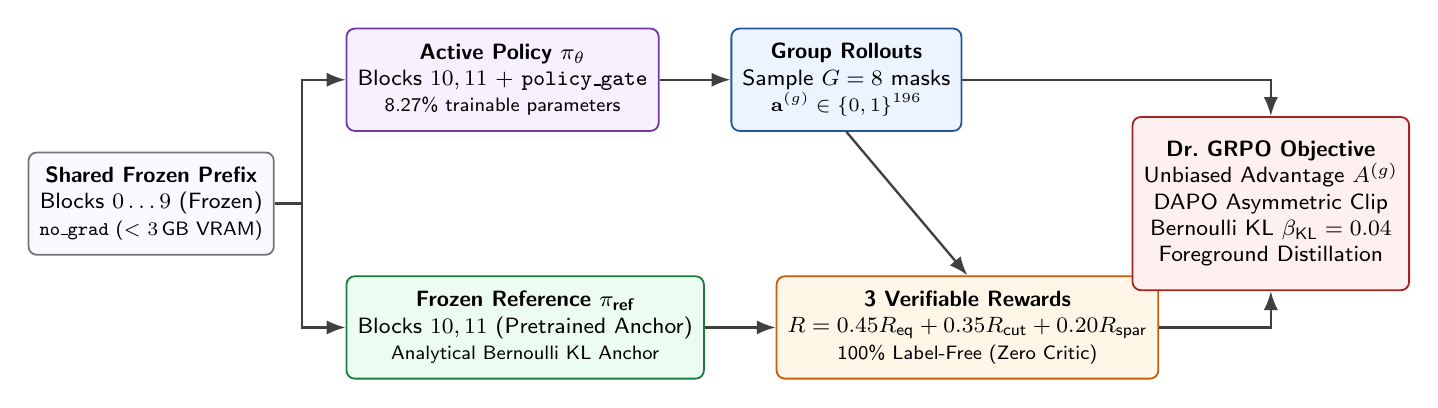
\begin{tikzpicture}[
    font=\sffamily\footnotesize,
    >=Latex,
    box/.style={draw=black!70, rounded corners=3pt, align=center, inner sep=4pt, line width=0.65pt},
    bluebox/.style={box, fill=softblue, draw=borderblue},
    greenbox/.style={box, fill=softgreen, draw=bordergreen},
    orangebox/.style={box, fill=softorange, draw=borderorange},
    purplebox/.style={box, fill=softpurple, draw=borderpurple},
    redbox/.style={box, fill=softred, draw=borderred},
    graybox/.style={box, fill=cardbg, draw=black!55},
    arrow/.style={->, line width=0.85pt, draw=black!75}
]
    % Shared Prefix
    \node[graybox, minimum width=2.6cm, minimum height=1.3cm] (prefix) {
        \textbf{Shared Frozen Prefix}\\
        Blocks $0\dots 9$ (Frozen)\\
        {\scriptsize \texttt{no\_grad} ($<3$\,GB VRAM)}
    };

    % Policy Net
    \node[purplebox, minimum width=3.2cm, minimum height=1.3cm, above right=0.25cm and 0.9cm of prefix] (policy) {
        \textbf{Active Policy $\pi_\theta$}\\
        Blocks $10, 11$ + \texttt{policy\_gate}\\
        {\scriptsize 8.27\% trainable parameters}
    };

    % Reference Net
    \node[greenbox, minimum width=3.2cm, minimum height=1.3cm, below right=0.25cm and 0.9cm of prefix] (ref) {
        \textbf{Frozen Reference $\pi_{\text{ref}}$}\\
        Blocks $10, 11$ (Pretrained Anchor)\\
        {\scriptsize Analytical Bernoulli KL Anchor}
    };

    % Rollouts
    \node[bluebox, minimum width=2.8cm, minimum height=1.3cm, right=0.9cm of policy] (rollout) {
        \textbf{Group Rollouts}\\
        Sample $G=8$ masks\\
        {\scriptsize $\mathbf{a}^{(g)} \in \{0, 1\}^{196}$}
    };

    % Verifiable Rewards
    \node[orangebox, minimum width=2.8cm, minimum height=1.3cm, right=0.9cm of ref] (rewards) {
        \textbf{3 Verifiable Rewards}\\
        $R = 0.45 R_{\text{eq}} + 0.35 R_{\text{cut}} + 0.20 R_{\text{spar}}$\\
        {\scriptsize 100\% Label-Free (Zero Critic)}
    };

    % Loss
    \coordinate (mid) at ($(rollout.east)!0.5!(rewards.east)$);
    \node[redbox, minimum width=3.2cm, minimum height=2.2cm, right=0.9cm of mid] (loss) {
        \textbf{Dr.\ GRPO Objective}\\
        Unbiased Advantage $A^{(g)}$\\
        DAPO Asymmetric Clip\\
        Bernoulli KL $\beta_{\text{KL}}=0.04$\\
        Foreground Distillation
    };

    \draw[arrow] (prefix.east) -- ++(0.35,0) |- (policy.west);
    \draw[arrow] (prefix.east) -- ++(0.35,0) |- (ref.west);
    \draw[arrow] (policy.east) -- (rollout.west);
    \draw[arrow] (ref.east) -- (rewards.west);
    \draw[arrow] (rollout.south) -- (rewards.north);
    \draw[arrow] (rollout.east) -| (loss.north);
    \draw[arrow] (rewards.east) -| (loss.south);
\end{tikzpicture}%
}

\vspace{0.3em}
\begin{columns}[t]
    \begin{column}{0.49\textwidth}
        \begin{block}{\textbf{Shared-Prefix Efficiency}}
            \small
            Freezing blocks $0\dots 9$ permits training on consumer hardware with \textbf{< 3\,GB VRAM}!
        \end{block}
    \end{column}

    \begin{column}{0.49\textwidth}
        \begin{exampleblock}{\textbf{Zero Neural Critic}}
            \small
            Eliminates value model entirely by estimating baselines directly from group rollouts ($G=8$).
        \end{exampleblock}
    \end{column}
\end{columns}
\end{frame}

% ==============================================================================
% SLIDE 8: VISUAL ANATOMY OF THE 3 VERIFIABLE REWARDS
% ==============================================================================
\begin{frame}{Visual Anatomy of the 3 Verifiable Visual Rewards}
\vspace{-0.3em}
\begin{columns}[t]
    % Reward 1: Equivariance
    \begin{column}{0.32\textwidth}
        \begin{block}{\textbf{1. Equivariance ($w=0.45$)}}
            \centering
            \vspace{0.2em}
            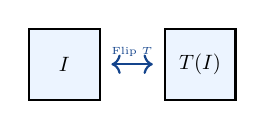
\begin{tikzpicture}[scale=0.75, every node/.style={transform shape}]
                \draw[thick, fill=softblue] (0,0) rectangle (1.2,1.2) node[pos=0.5] {$I$};
                \draw[<->, thick, accentblue] (1.4,0.6) -- node[above, font=\tiny] {Flip $T$} (2.1,0.6);
                \draw[thick, fill=softblue] (2.3,0.0) rectangle (3.5,1.2) node[pos=0.5] {$T(I)$};
            \end{tikzpicture}
            \vspace{0.2em}
            \footnotesize
            \textbf{Horizontal-Flip Consistency}:
            \[ R_{\text{equiv}} = \text{IoU}\big(\mathbf{a}^{(g)}, \, \mathbf{m}_{\text{eq}}\big) \]
            Blended with unsupervised spectral-contour pseudo-mask.
        \end{block}
    \end{column}

    % Reward 2: TokenCut Compactness
    \begin{column}{0.32\textwidth}
        \begin{block}{\textbf{2. Compactness ($w=0.35$)}}
            \centering
            \vspace{0.2em}
            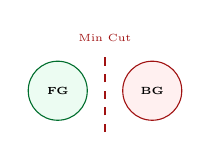
\begin{tikzpicture}[scale=0.75, every node/.style={transform shape}]
                \draw[fill=softgreen, draw=darkgreen] (0.6,0.6) circle (0.5cm) node[font=\tiny\bfseries] {FG};
                \draw[fill=softred, draw=crimsonred] (2.2,0.6) circle (0.5cm) node[font=\tiny\bfseries] {BG};
                \draw[dashed, thick, crimsonred] (1.4,-0.1) -- (1.4,1.3) node[above, font=\tiny] {Min Cut};
            \end{tikzpicture}
            \vspace{0.2em}
            \footnotesize
            \textbf{Graph-Spectral TokenCut}:
            \[ R_{\text{comp}} = 0.65 S_{\text{NCut}} + 0.35(1 - \text{TV}) \]
            Maximizes intra-object affinity while penalizing boundary fragmentation.
        \end{block}
    \end{column}

    % Reward 3: Sparsity Prior
    \begin{column}{0.32\textwidth}
        \begin{block}{\textbf{3. Sparsity ($w=0.20$)}}
            \centering
            \vspace{0.2em}
            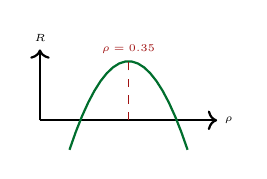
\begin{tikzpicture}[scale=0.75, every node/.style={transform shape}]
                \draw[->, thick] (0,0) -- (3.0,0) node[right, font=\tiny] {$\rho$};
                \draw[->, thick] (0,0) -- (0,1.2) node[above, font=\tiny] {$R$};
                \draw[thick, darkgreen] plot[domain=0.5:2.5, samples=20] (\x, {1.0 - 1.5*(\x-1.5)*(\x-1.5)});
                \draw[dashed, crimsonred] (1.5,0) -- (1.5,1.0) node[above, font=\tiny] {$\rho=0.35$};
            \end{tikzpicture}
            \vspace{0.2em}
            \footnotesize
            \textbf{Target Ratio Prior}:
            \[ R_{\text{spar}} = \max\left(0, 1 - \left|\tfrac{\bar{a} - 0.35}{0.65}\right|^{1.5}\right) \]
            Strictly prevents trivial all-foreground or empty masks.
        \end{block}
    \end{column}
\end{columns}

\vspace{0.3em}
\begin{exampleblock}{\textbf{100\% Verifiable Scientific Guarantee}}
    \centering\small
    Zero neural reward models $\implies$ immune to reward hacking or adversarial policy drift!
\end{exampleblock}
\end{frame}

% ==============================================================================
% SLIDE 9: DR. GRPO ADVANTAGE & CONVERGENCE DYNAMICS
% ==============================================================================
\begin{frame}{Dr.\ GRPO Unbiased Advantage \& Convergence Dynamics}
\vspace{-0.3em}
\begin{columns}[c]
    % Visual diagram of Unbiased Advantage
    \begin{column}{0.48\textwidth}
        \begin{block}{\textbf{Unbiased Group Advantage $A^{(g)}$}}
            \centering
            \vspace{0.2em}
            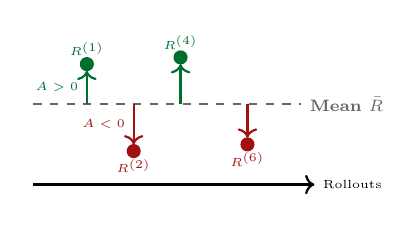
\begin{tikzpicture}[scale=0.85, every node/.style={transform shape}]
                \draw[->, thick] (0,0) -- (4.2,0) node[right, font=\tiny] {Rollouts};
                \draw[dashed, thick, black!60] (0,1.2) -- (4.0,1.2) node[right, font=\scriptsize\bfseries] {Mean $\bar{R}$};
                
                % Rollouts above
                \fill[darkgreen] (0.8, 1.8) circle (3pt) node[above, font=\tiny\bfseries] {$R^{(1)}$};
                \draw[->, thick, darkgreen] (0.8, 1.2) -- (0.8, 1.7) node[pos=0.5, left, font=\tiny] {$A > 0$};
                \fill[darkgreen] (2.2, 1.9) circle (3pt) node[above, font=\tiny\bfseries] {$R^{(4)}$};
                \draw[->, thick, darkgreen] (2.2, 1.2) -- (2.2, 1.8);

                % Rollouts below
                \fill[crimsonred] (1.5, 0.5) circle (3pt) node[below, font=\tiny\bfseries] {$R^{(2)}$};
                \draw[->, thick, crimsonred] (1.5, 1.2) -- (1.5, 0.6) node[pos=0.5, left, font=\tiny] {$A < 0$};
                \fill[crimsonred] (3.2, 0.6) circle (3pt) node[below, font=\tiny\bfseries] {$R^{(6)}$};
                \draw[->, thick, crimsonred] (3.2, 1.2) -- (3.2, 0.7);
            \end{tikzpicture}
            \vspace{0.2em}
            \scriptsize
            \textbf{Why Dr.\ GRPO?}: Omitting $\sigma_R$ division eliminates gradient explosions when all rollouts achieve similar rewards!
        \end{block}
    \end{column}

    % Convergence Chart
    \begin{column}{0.50\textwidth}
        \begin{exampleblock}{\textbf{10-Epoch Monotonic Convergence}}
            \centering
            \vspace{0.2em}
            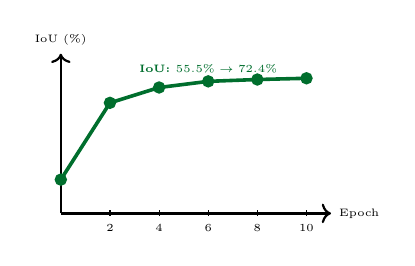
\begin{tikzpicture}[scale=0.78, every node/.style={transform shape}]
                \draw[->, thick] (0,0) -- (4.4,0) node[right, font=\tiny] {Epoch};
                \draw[->, thick] (0,0) -- (0,2.6) node[above, font=\tiny] {IoU (\%)};
                \foreach \x/\v in {0.8/2, 1.6/4, 2.4/6, 3.2/8, 4.0/10} {
                    \draw (\x, 0.05) -- (\x, -0.05) node[below, font=\tiny] {\v};
                }
                % IoU Curve
                \draw[line width=1.3pt, darkgreen, mark=*] plot coordinates {
                    (0.0, 0.55) (0.8, 1.80) (1.6, 2.05) (2.4, 2.15) (3.2, 2.18) (4.0, 2.20)
                };
                \node[font=\tiny\bfseries, text=darkgreen] at (2.4, 2.35) {IoU: $55.5\% \to 72.4\%$};
            \end{tikzpicture}
            \vspace{0.2em}
            \scriptsize
            Rapid, monotonic improvement within 2 epochs; zero policy collapse or catastrophic forgetting!
        \end{exampleblock}
    \end{column}
\end{columns}
\end{frame}

% ==============================================================================
% SLIDE 10: QUANTITATIVE BENCHMARK: CIFAR-10 CLASSIFICATION
% ==============================================================================
\begin{frame}{Quantitative Benchmark: CIFAR-10 Downstream Evaluation}
\vspace{-0.3em}
Downstream evaluation of backbones pretrained for 190 epochs on \textbf{ImageNet-100}:

\vspace{0.1em}
\centering
\small
\begin{tabular}{lccc}
\toprule
\textbf{Metric} & \textbf{Baseline ViT-Small} & \textbf{Dr.\ DINO (Ours)} & \textbf{Gain ($\Delta$)} \\
\midrule
$k$-NN Top-1 ($k=10$) & 74.41\% & \textbf{75.97\%} & \textcolor{darkgreen}{\textbf{+1.56\%}} \\
$k$-NN Top-1 ($k=20$) & 74.34\% & \textbf{75.31\%} & \textcolor{darkgreen}{\textbf{+0.97\%}} \\
$k$-NN Top-1 ($k=200$) & 70.41\% & \textbf{70.65\%} & \textcolor{darkgreen}{\textbf{+0.24\%}} \\
\midrule
Linear Probe Top-1 (Epoch 10) & 80.92\% & \textbf{83.38\%} & \textcolor{darkgreen}{\textbf{+2.46\%}} \\
Linear Probe Top-1 (Epoch 30) & 80.85\% & \textbf{83.63\%} & \textcolor{darkgreen}{\textbf{+2.78\%}} \\
Linear Probe Top-1 (\textbf{Best Checkpoint}) & 81.46\% & \textbf{83.98\%} & \textcolor{darkgreen}{\textbf{+2.52\%}} \\
Linear Probe Top-5 (\textbf{Best Checkpoint}) & 99.31\% & \textbf{99.44\%} & \textcolor{darkgreen}{\textbf{+0.13\%}} \\
\bottomrule
\end{tabular}

\vspace{0.4em}
\begin{columns}[t]
    \begin{column}{0.49\textwidth}
        \begin{block}{\textbf{Rapid Linear Convergence}}
            \small
            By \textbf{Epoch 10}, Dr.\ DINO reaches \textbf{83.38\%}, already beating the baseline's 100-epoch peak (\textbf{81.46\%})!
        \end{block}
    \end{column}

    \begin{column}{0.49\textwidth}
        \begin{exampleblock}{\textbf{Exact Zero Capacity Inflation}}
            \small
            Both backbones have \textbf{21,665,664} parameters and \textbf{9.20 GFLOPs} ($\Delta = 0$). Gains stem purely from geometric bias.
        \end{exampleblock}
    \end{column}
\end{columns}
\end{frame}

% ==============================================================================
% SLIDE 11: VISUAL EVIDENCE I: STAGE-1 ATTENTION SPECIALIZATION (NO RLVR YET)
% ==============================================================================
\begin{frame}{Visual Evidence I: Stage-1 Multi-Head Attention Specialization}
\vspace{-0.4em}
\begin{columns}[c]
    \begin{column}{0.62\textwidth}
        \begin{block}{\textbf{Airplane: Fuselage \& Wings vs.\ Sky Clutter (Stage 1)}}
            \centering
            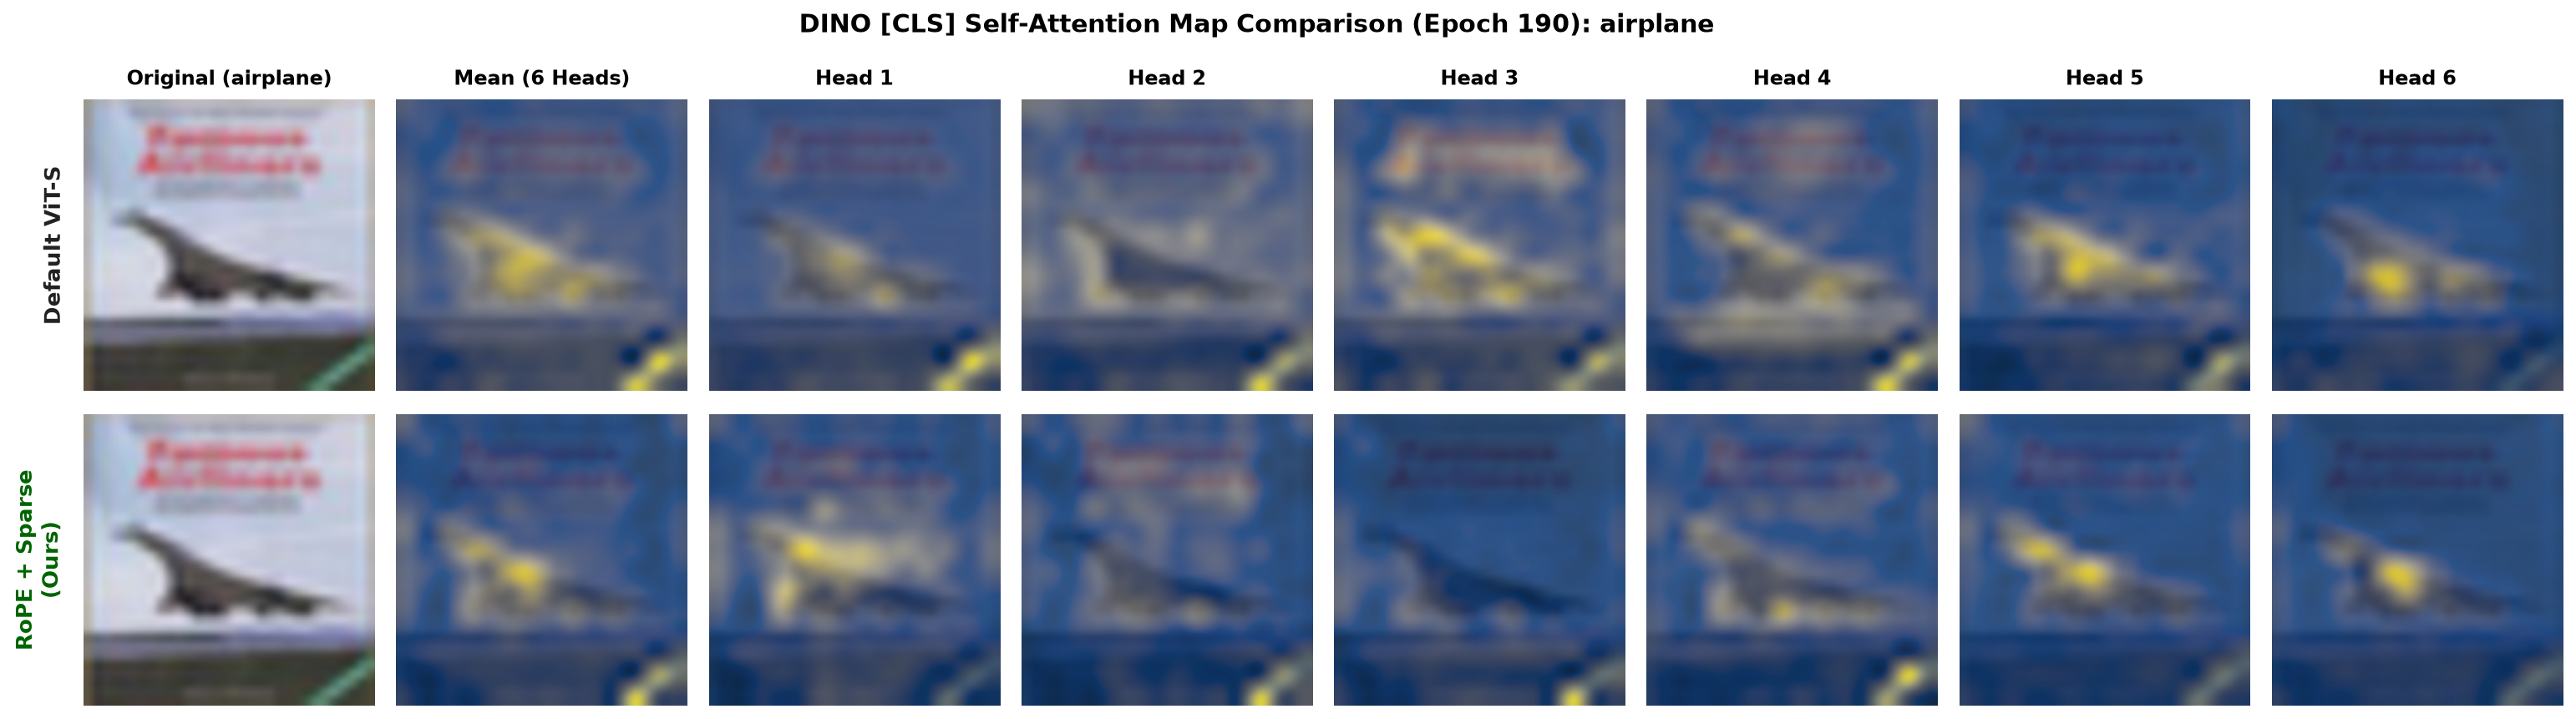
\includegraphics[width=\linewidth, height=0.24\textheight, keepaspectratio]{output/attention_comparison.png}
        \end{block}
        \vspace{-0.6em}
        \begin{block}{\textbf{Horse: Muscle Contours vs.\ Turf Bleed (Stage 1)}}
            \centering
            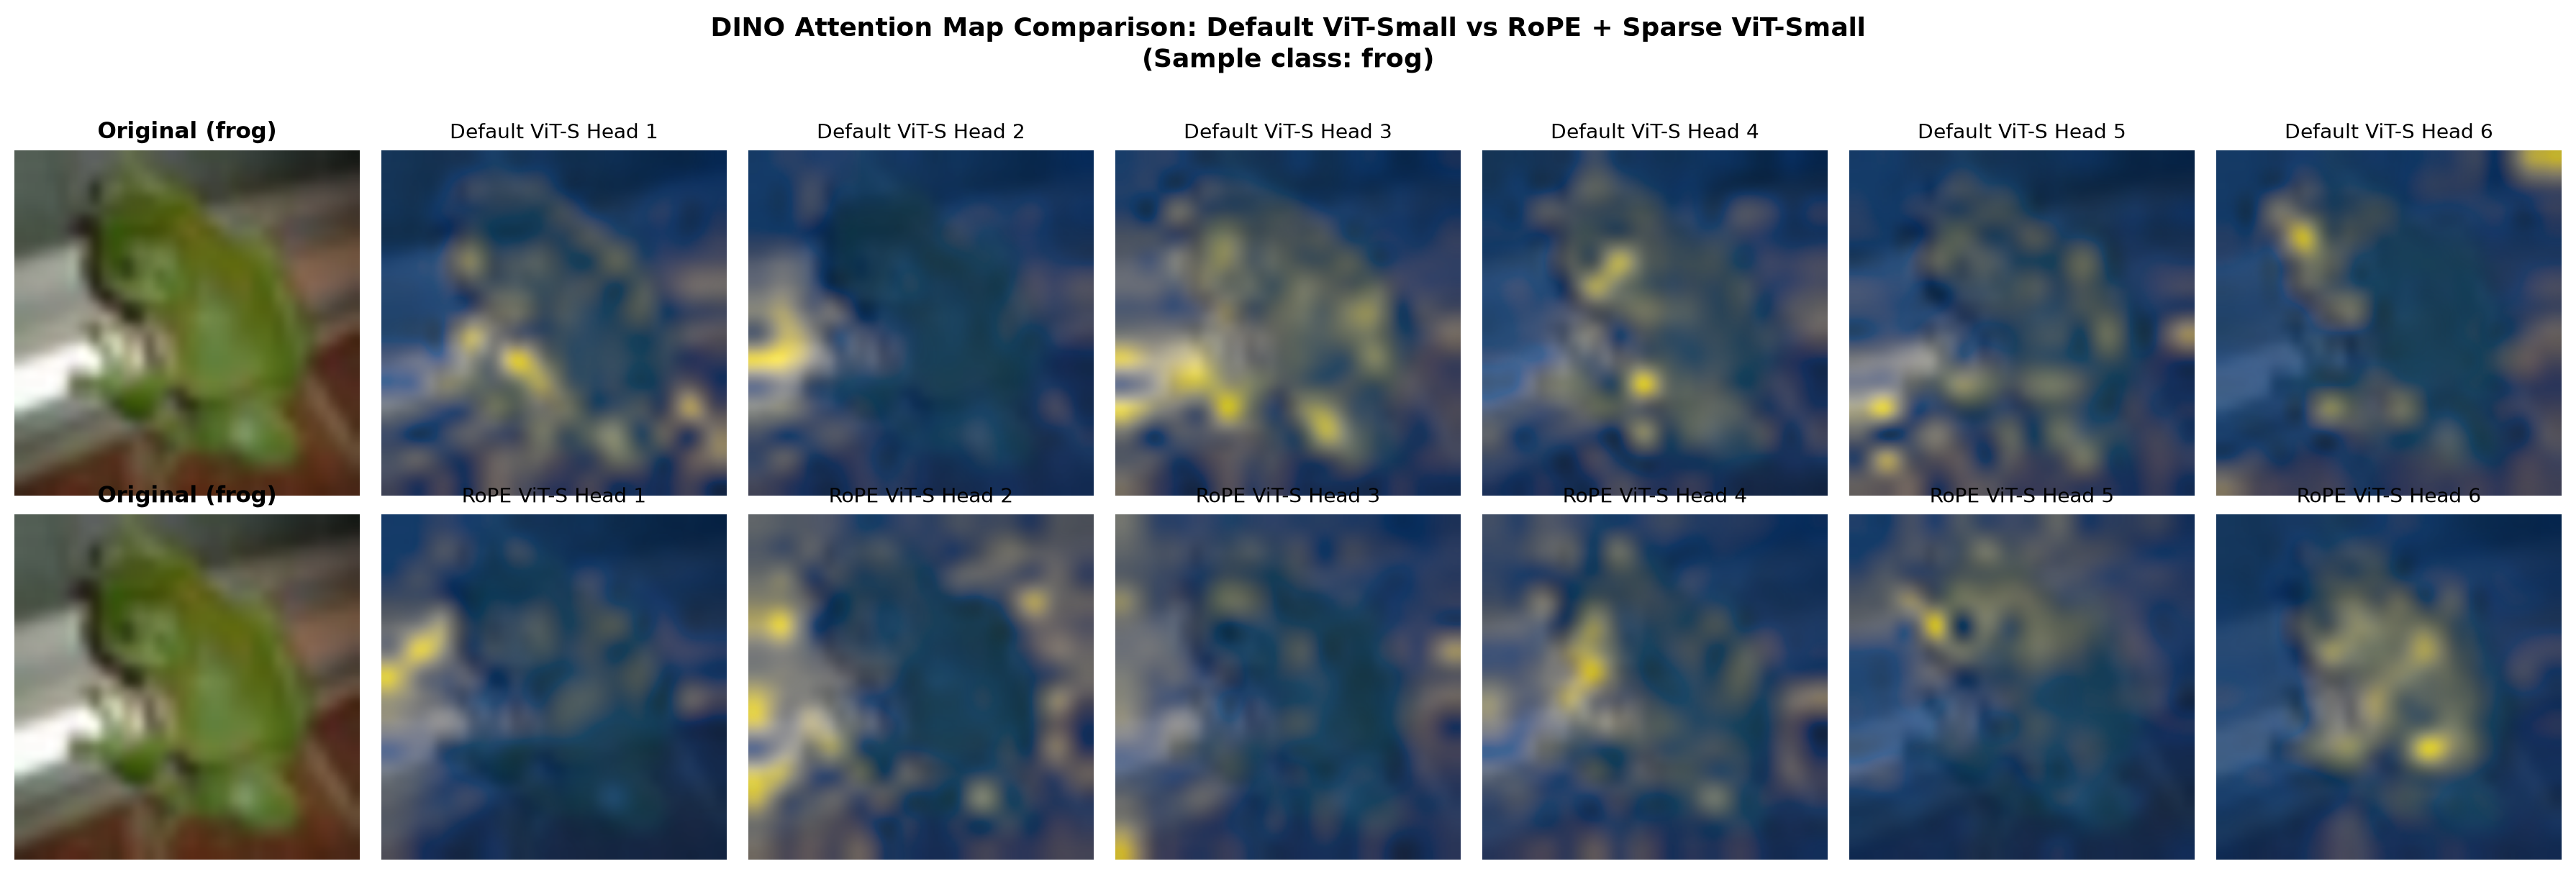
\includegraphics[width=\linewidth, height=0.24\textheight, keepaspectratio]{output/attention_comparison_horse.png}
        \end{block}
    \end{column}

    \begin{column}{0.35\textwidth}
        \begin{exampleblock}{\textbf{Stage-1 Specialization}}
            \small
            \begin{itemize}\setlength{\itemsep}{2pt}
                \item \textbf{Baseline ViT}: Heads 1, 3, 4 diffuse mass onto sky and grass.
                \item \textbf{Dr.\ DINO-Base}: Heads 2 and 5 lock sharply onto physical structures.
                \item \textbf{No RLVR Yet}: Stage-1 backbones evaluated prior to Dr.\ GRPO post-training.
            \end{itemize}
        \end{exampleblock}
    \end{column}
\end{columns}
\end{frame}

% ==============================================================================
% SLIDE 12: COMPLETE 2x2 FACTORIAL ABLATION MATRIX
% ==============================================================================
\begin{frame}{Complete $2 \times 2$ Factorial Ablation Matrix}
\vspace{-0.3em}
Evaluated on full CIFAR-10 (50,000 train / 10,000 test images) across both axes:

\vspace{0.1em}
\centering
\small
\resizebox{\textwidth}{!}{%
\begin{tabular}{llccccc}
\toprule
\textbf{Model Variant} & \textbf{Backbone Arch} & \textbf{Dr.\ GRPO} & \textbf{$k$-NN Top-1} & \textbf{Linear Probe} & \textbf{Mask IoU} & \textbf{CorLoc} \\
\midrule
1. Vanilla DINOv1 & \texttt{vit\_small} & No & 71.13\% & 78.07\% & 58.88\% & 79.93\% \\
2. Dr.\ DINO-Base & \texttt{vit\_small\_sparse\_rope} & No & 71.83\% & 80.22\% & 55.45\% & 69.26\% \\
3. Vanilla + Dr.\ GRPO & \texttt{vit\_small} & Yes & 71.29\% & 78.44\% & \textbf{78.98\%} & \textbf{99.91\%} \\
\textbf{4. Dr.\ DINO-Full (Ours)} & \texttt{vit\_small\_sparse\_rope} & \textbf{Yes} & \textbf{72.05\%} & \textbf{80.67\%} & \textbf{72.44\%} & \textbf{98.17\%} \\
\bottomrule
\end{tabular}%
}

\vspace{0.3em}
\begin{columns}[t]
    \begin{column}{0.49\textwidth}
        \begin{alertblock}{\textbf{Massive Object Discovery Surge}}
            \small
            \begin{itemize}\setlength{\itemsep}{1pt}
                \item \textbf{+20.10\%} Mask IoU on Vanilla ($58.88\% \to 78.98\%$).
                \item \textbf{+16.99\%} Mask IoU on Dr.\ DINO ($55.45\% \to 72.44\%$).
                \item \textbf{CorLoc reaches 99.91\%} without any labels!
            \end{itemize}
        \end{alertblock}
    \end{column}

    \begin{column}{0.49\textwidth}
        \begin{exampleblock}{\textbf{Synergistic Downstream Gains}}
            \small
            \begin{itemize}\setlength{\itemsep}{1pt}
                \item \textbf{No Catastrophic Forgetting}: Downstream Linear Probe improves (+0.45\% to \textbf{80.67\%}).
                \item Top $k$-NN accuracy (\textbf{72.05\%}) across all 4 variants!
            \end{itemize}
        \end{exampleblock}
    \end{column}
\end{columns}
\end{frame}

% ==============================================================================
% SLIDE 13: VISUAL EVIDENCE II: 2x2 QUALITATIVE GRID
% ==============================================================================
\begin{frame}{Visual Evidence II: Unsupervised Object Discovery Gallery}
\vspace{-0.3em}
\centering
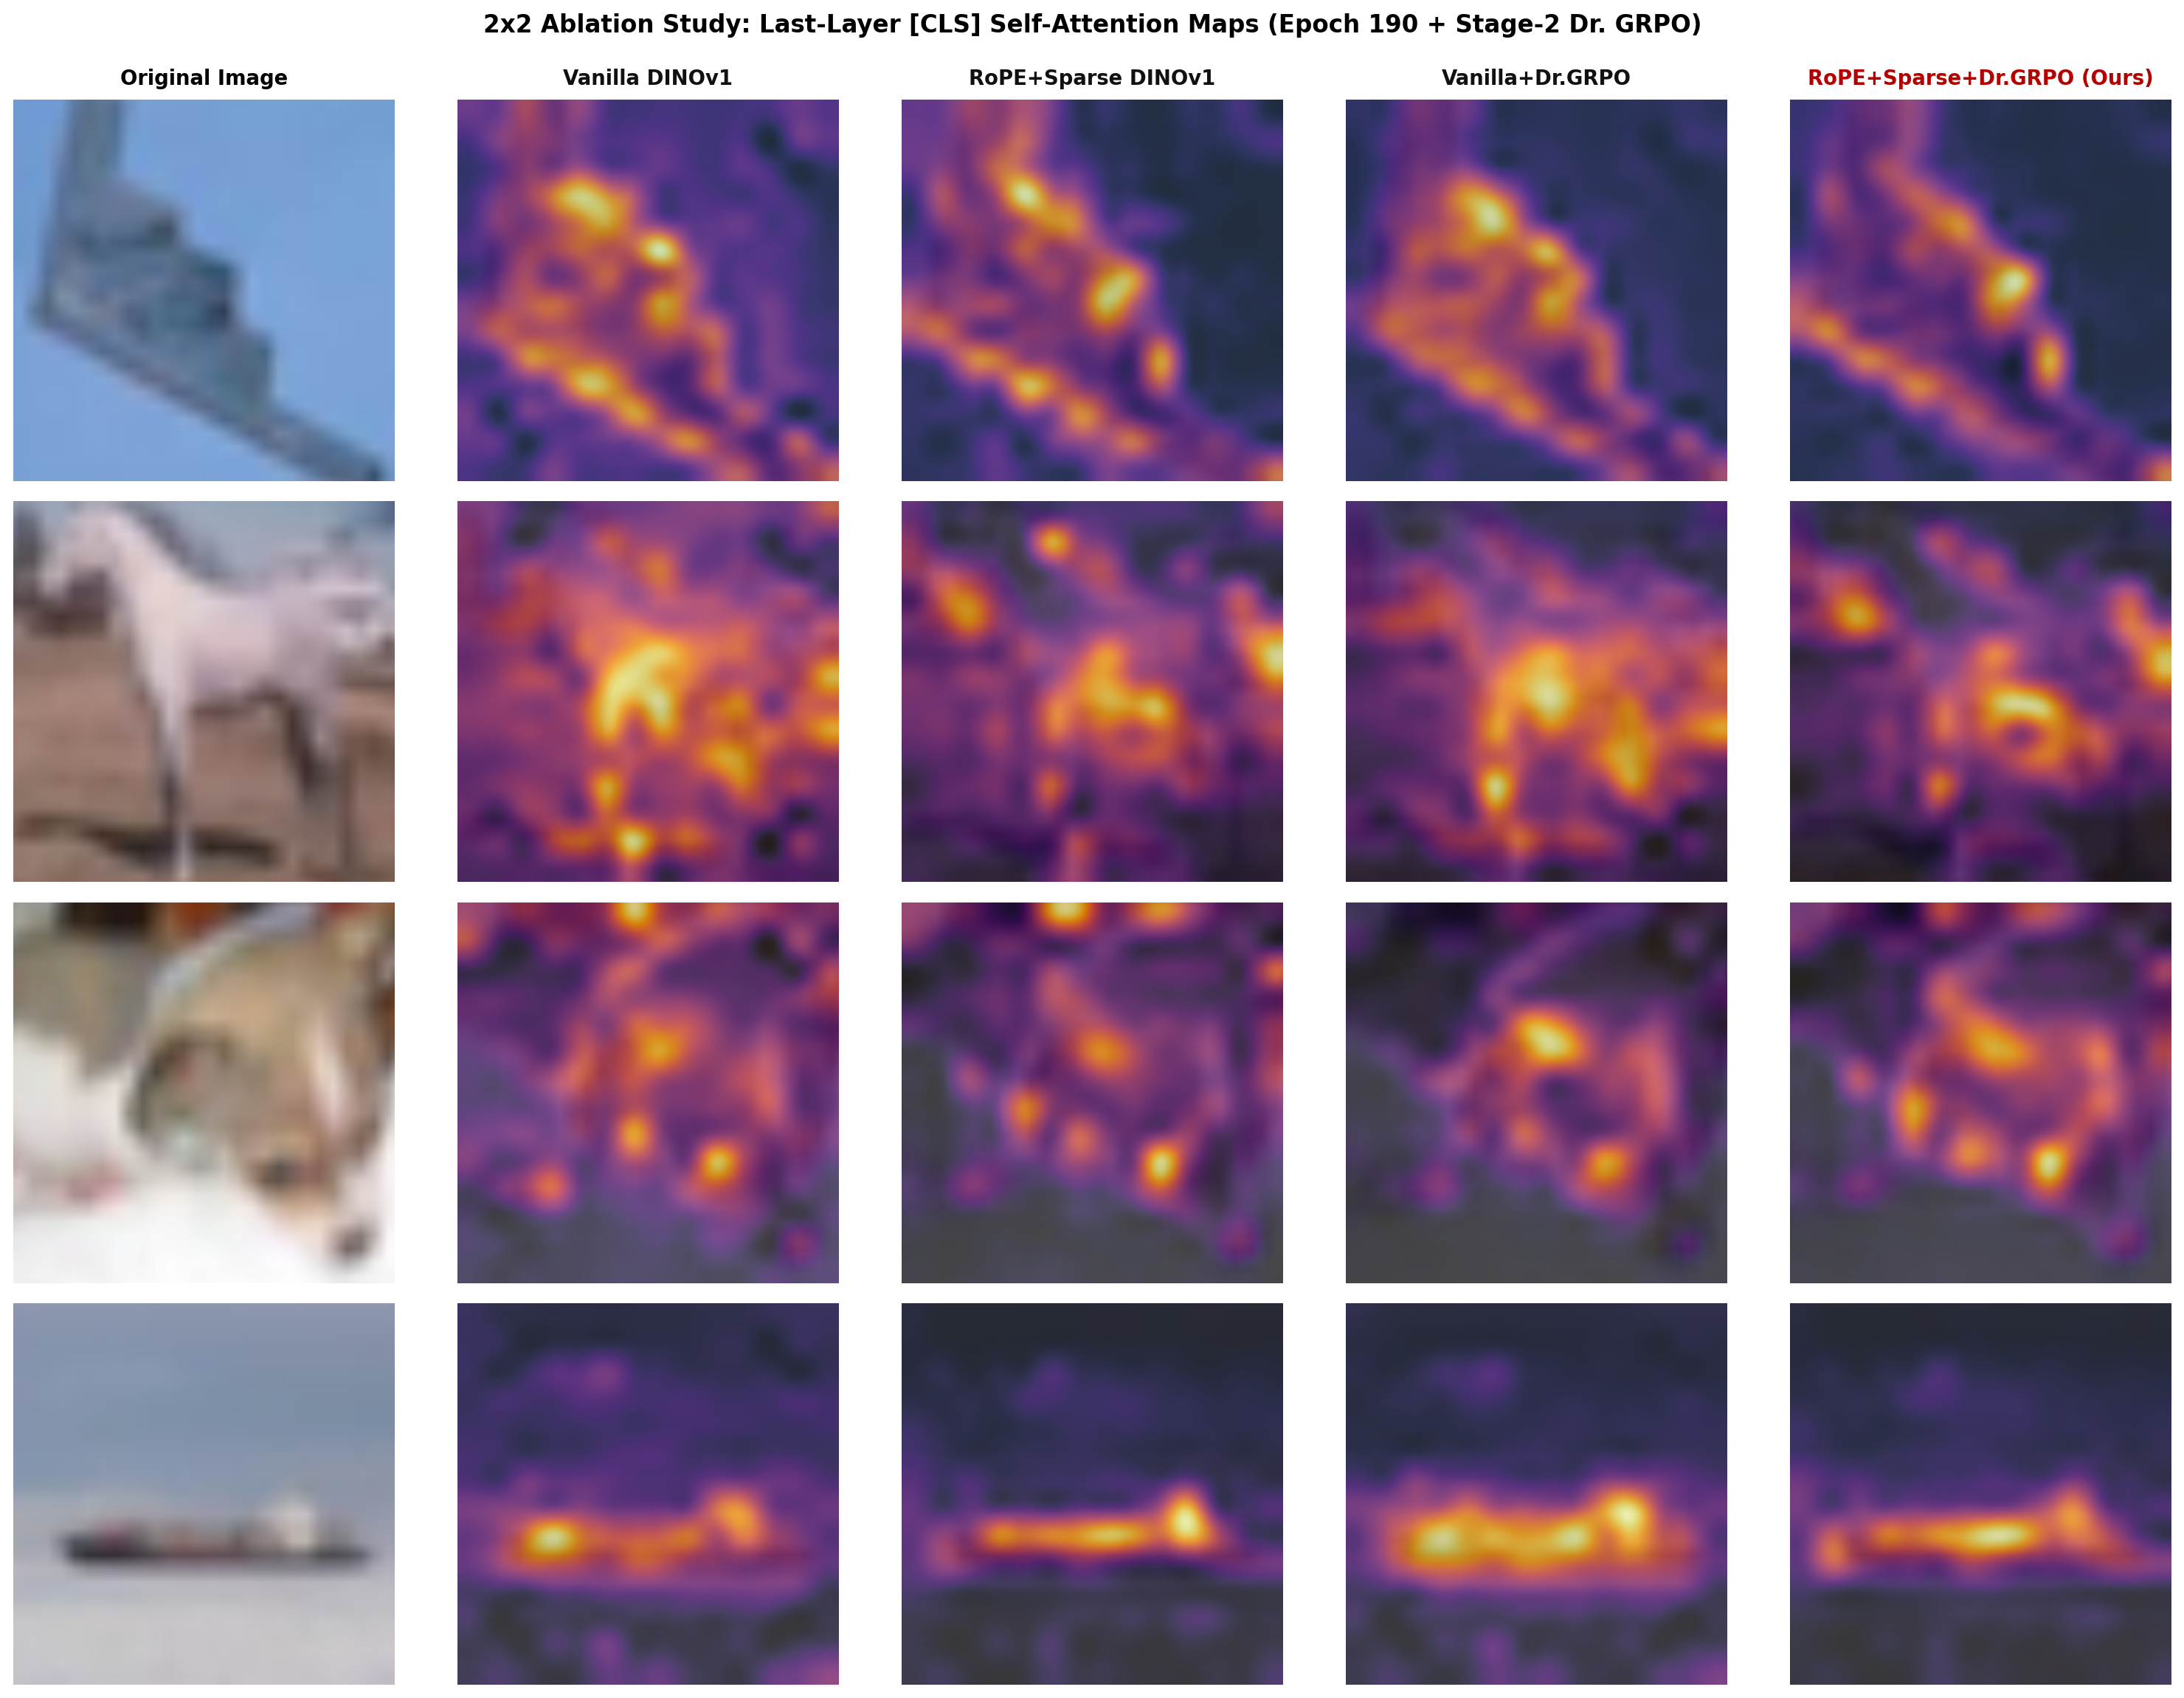
\includegraphics[height=0.62\textheight, keepaspectratio]{output/ablation_2x2_attention_grid.png}

\vspace{-0.2em}
\begin{exampleblock}{\textbf{Qualitative Proof of Background Noise Suppression}}
    \centering\footnotesize
    \textbf{Original Image} $\implies$ \textbf{Vanilla DINO} (Halos) $\implies$ \textbf{Dr.\ DINO-Base} (Sub-parts) $\implies$ \textbf{Vanilla+Dr.GRPO} $\implies$ \textbf{Dr.\ DINO-Full} (Precise Mask)
\end{exampleblock}
\end{frame}

% ==============================================================================
% SLIDE 14: HARDWARE PROFILING & EFFICIENCY
% ==============================================================================
\begin{frame}{Hardware Profiling \& Computational Efficiency}
\vspace{-0.3em}
Benchmarked at $224 \times 224$ input resolution on an \textbf{NVIDIA RTX 3070 GPU}:

\vspace{0.1em}
\centering
\small
\resizebox{0.95\textwidth}{!}{%
\begin{tabular}{lccc}
\toprule
\textbf{Resource Metric} & \textbf{Baseline ViT-Small} & \textbf{Dr.\ DINO (Ours)} & \textbf{Comparison} \\
\midrule
Backbone Trainable Parameters & 21,665,664 & 21,665,664 & \textbf{0\% Overhead (Identical)} \\
Projection Head Parameters & 9,720,064 & 9,720,064 & Identical \\
\textbf{Total Model Parameters} & \textbf{31,385,728} & \textbf{31,385,728} & \textbf{31.39M (Identical)} \\
\midrule
Theoretical FLOPs per Image & 9.22 GFLOPs & 9.22 GFLOPs & \textbf{Exact Parity (4.60 GMACs)} \\
Active Attention Pairs per Token & 197 keys & \textbf{26 keys} & \textbf{$-86.8\%$ Sparsity Savings} \\
Inference Latency (BS=1) & 1.20 ms & 2.20 ms & +1.00 ms (PyTorch RoPE) \\
RLVR Policy VRAM Footprint & -- & \textbf{< 3\,GB} & \textbf{Shared-Prefix Efficiency} \\
\bottomrule
\end{tabular}%
}

\vspace{0.4em}
\begin{block}{\textbf{Key Engineering Takeaway}}
    \centering\small
    Dr.\ DINO proves that advanced self-supervised vision models and RLVR post-training can be trained and evaluated efficiently on \textbf{consumer-grade GPUs} (<3\,GB VRAM).
\end{block}
\end{frame}

% ==============================================================================
% SLIDE 15: CONCLUSION & DEFENSE TAKEAWAYS
% ==============================================================================
\begin{frame}{Conclusion: Three Pillars of Dr.\ DINO}
\vspace{-0.3em}
\begin{columns}[t]
    \begin{column}{0.32\textwidth}
        \begin{block}{\textbf{1. 2D RoPE Geometry}}
            \small
            \begin{itemize}\setlength{\itemsep}{2pt}
                \item Continuous 2D rotation.
                \item Frequency-spectrum ramp.
                \item Eliminates multi-crop bicubic distortion.
            \end{itemize}
        \end{block}
    \end{column}

    \begin{column}{0.32\textwidth}
        \begin{block}{\textbf{2. Structured Sparsity}}
            \small
            \begin{itemize}\setlength{\itemsep}{2pt}
                \item Chebyshev $3\times 3$ + Top-$16$ + \texttt{[CLS]}.
                \item $-86.8\%$ key pairs.
                \item Exact Softmax normalization.
            \end{itemize}
        \end{block}
    \end{column}

    \begin{column}{0.32\textwidth}
        \begin{exampleblock}{\textbf{3. Verifiable Dr.\ GRPO}}
            \small
            \begin{itemize}\setlength{\itemsep}{2pt}
                \item Unbiased RLVR advantages.
                \item +20.10\% Foreground Mask IoU.
                \item Reaches \textbf{99.91\% CorLoc} without human labels!
            \end{itemize}
        \end{exampleblock}
    \end{column}
\end{columns}

\vspace{0.4em}
\begin{center}
    \statbadge{Dr.\ DINO: Verifiable RLVR Discovery}{navyblue}{M.Sc. in Data Science -- HCMUS}\\[0.4em]
    \Large\textbf{Thank you for your attention!} \\[0.2em]
    \normalsize Questions \& Discussion
\end{center}
\end{frame}

\end{document}
